%----------------------------------------------------------------------------
%----------------------------------------------------------------------------
%----------------------------------------------------------------------------
%bb defines the bounding box for the pdf
%viewport defines the area of the pdf used
%in sidewaysfigure the last entry in bb moves the caption toward/away the pic
%in sidewaysfigure the second entry in bb moves the pic toward/away the caption
%----------------------------------------------------------------------------
\begin{figure}
\scalebox{0.8}[0.8]{
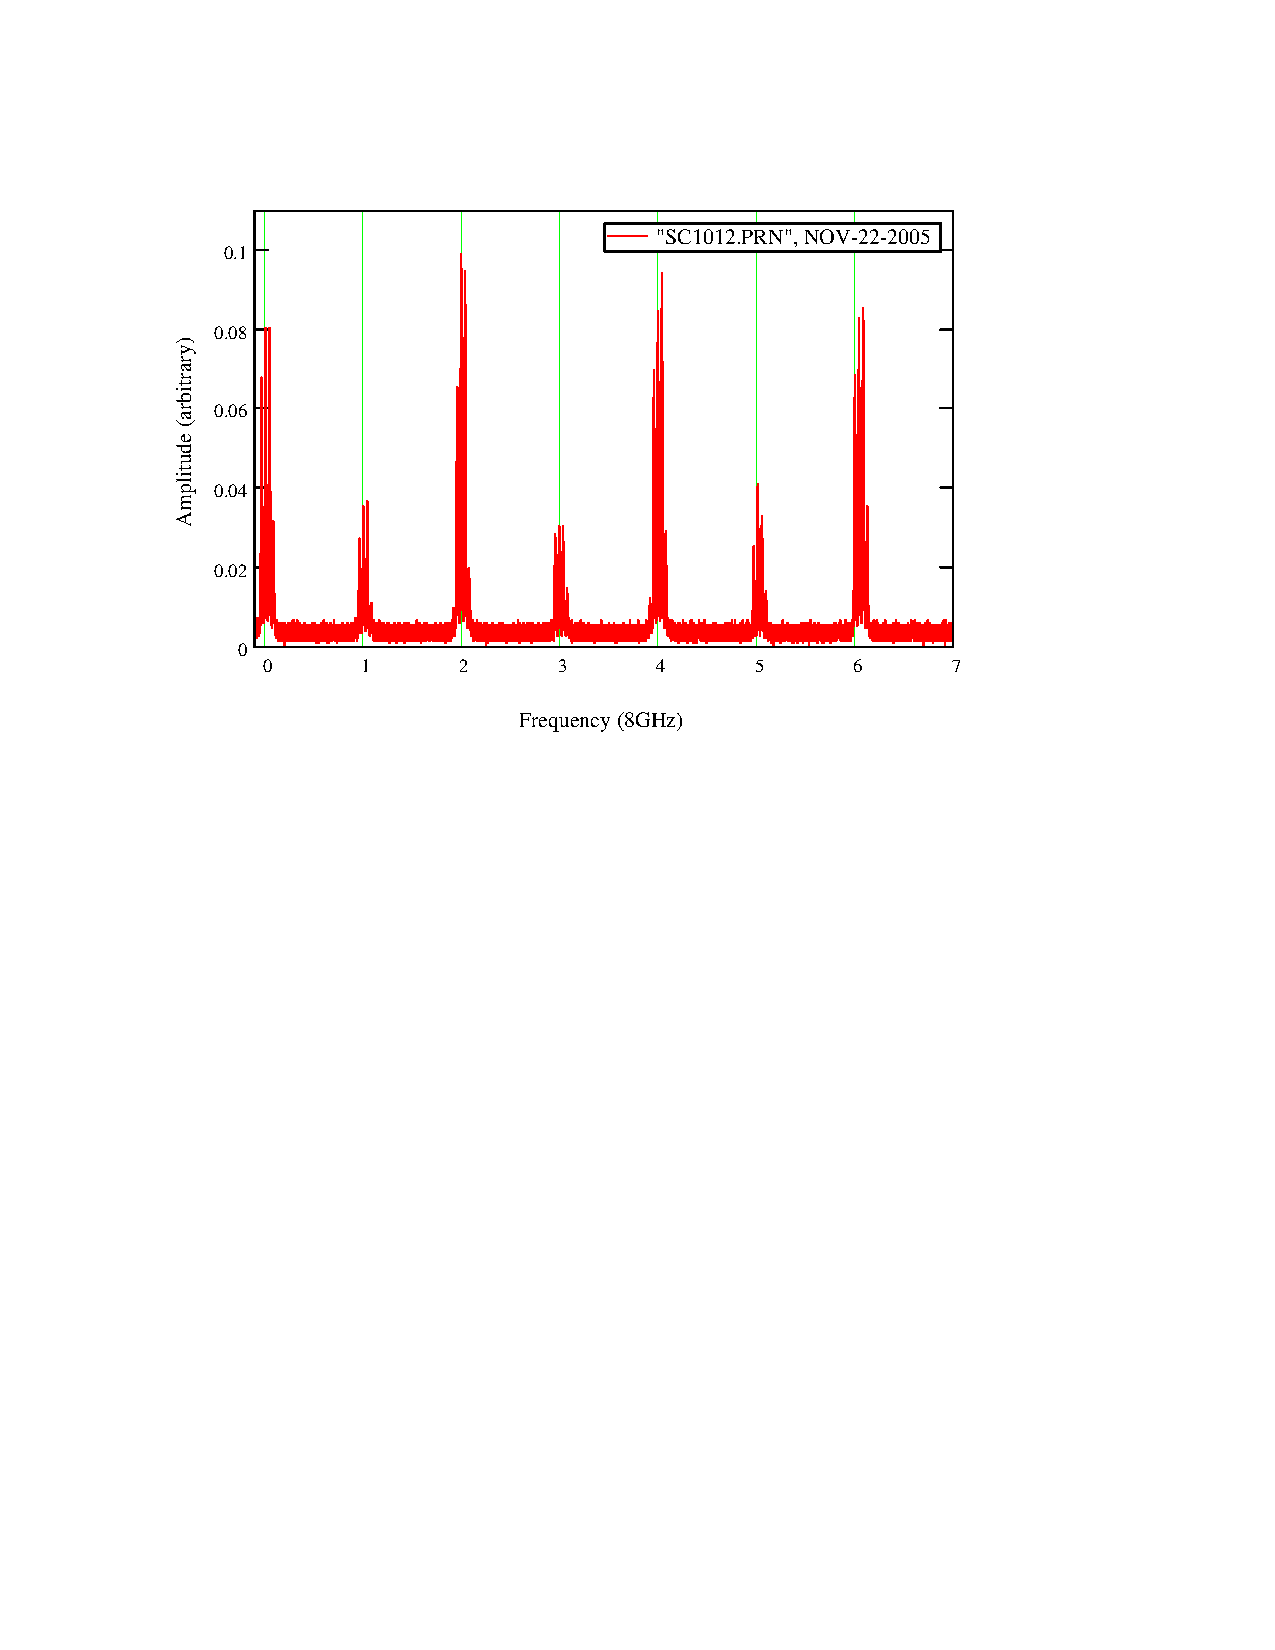
\includegraphics[bb=15 440 489 752]
{confocal_all/confocal_all.pdf}
}
\caption[Green HeNe transmission through a scanned confocal etalon]{Green HeNe transmission through a scanned confocal etalon}
\label{confocal_all}
\end{figure}
%----------------------------------------------------------------------------

%----------------------------------------------------------------------------
The Burleigh SA--Plus confocal etalon is tested on green HeNe output. This etalon is designed for laser beam analysis; however, in this test we attempt to investigate the possibility of using this type of etalon as a spectral filter for the dye laser output.

The output of a green HeNe is collimated using a telescope. The resulting beam is directed to the input of the confocal etalon. Careful alignment is required for optimal performance so a mount is assembled giving the proper number of adjustable parameters. The output of the etalon is then collected with a positive lens and focused onto the sensitive area of a photodiode. The diode is viewed on a digital oscilloscope which also provides a storage function so that scope traces can be easily transported to a computer.

The rear mirror of the etalon is allowed to translate under the action of a piezo actuator. Translating the cavity mirror essentially ``sweeps'' the comb band pass function of the etalon across the (stationary) laser line. If a voltage ramp is used to drive the piezo and the scope sweep, periodic maxima appear corresponding to each comb ``tooth'' that passes over the laser line. The mode spacing in the etalon used here is 8 GHz (this is half of the FSR since the etalon is confocal \cite{Siegman:1986a}) thus the scans can be calibrated as long as two maxima appear.

%----------------------------------------------------------------------------
%----------------------------------------------------------------------------
%bb defines the bounding box for the pdf
%viewport defines the area of the pdf used
%in sidewaysfigure the last entry in bb moves the caption toward/away the pic
%in sidewaysfigure the second entry in bb moves the pic toward/away the caption
%----------------------------------------------------------------------------
\begin{figure}
\scalebox{0.8}[0.8]{
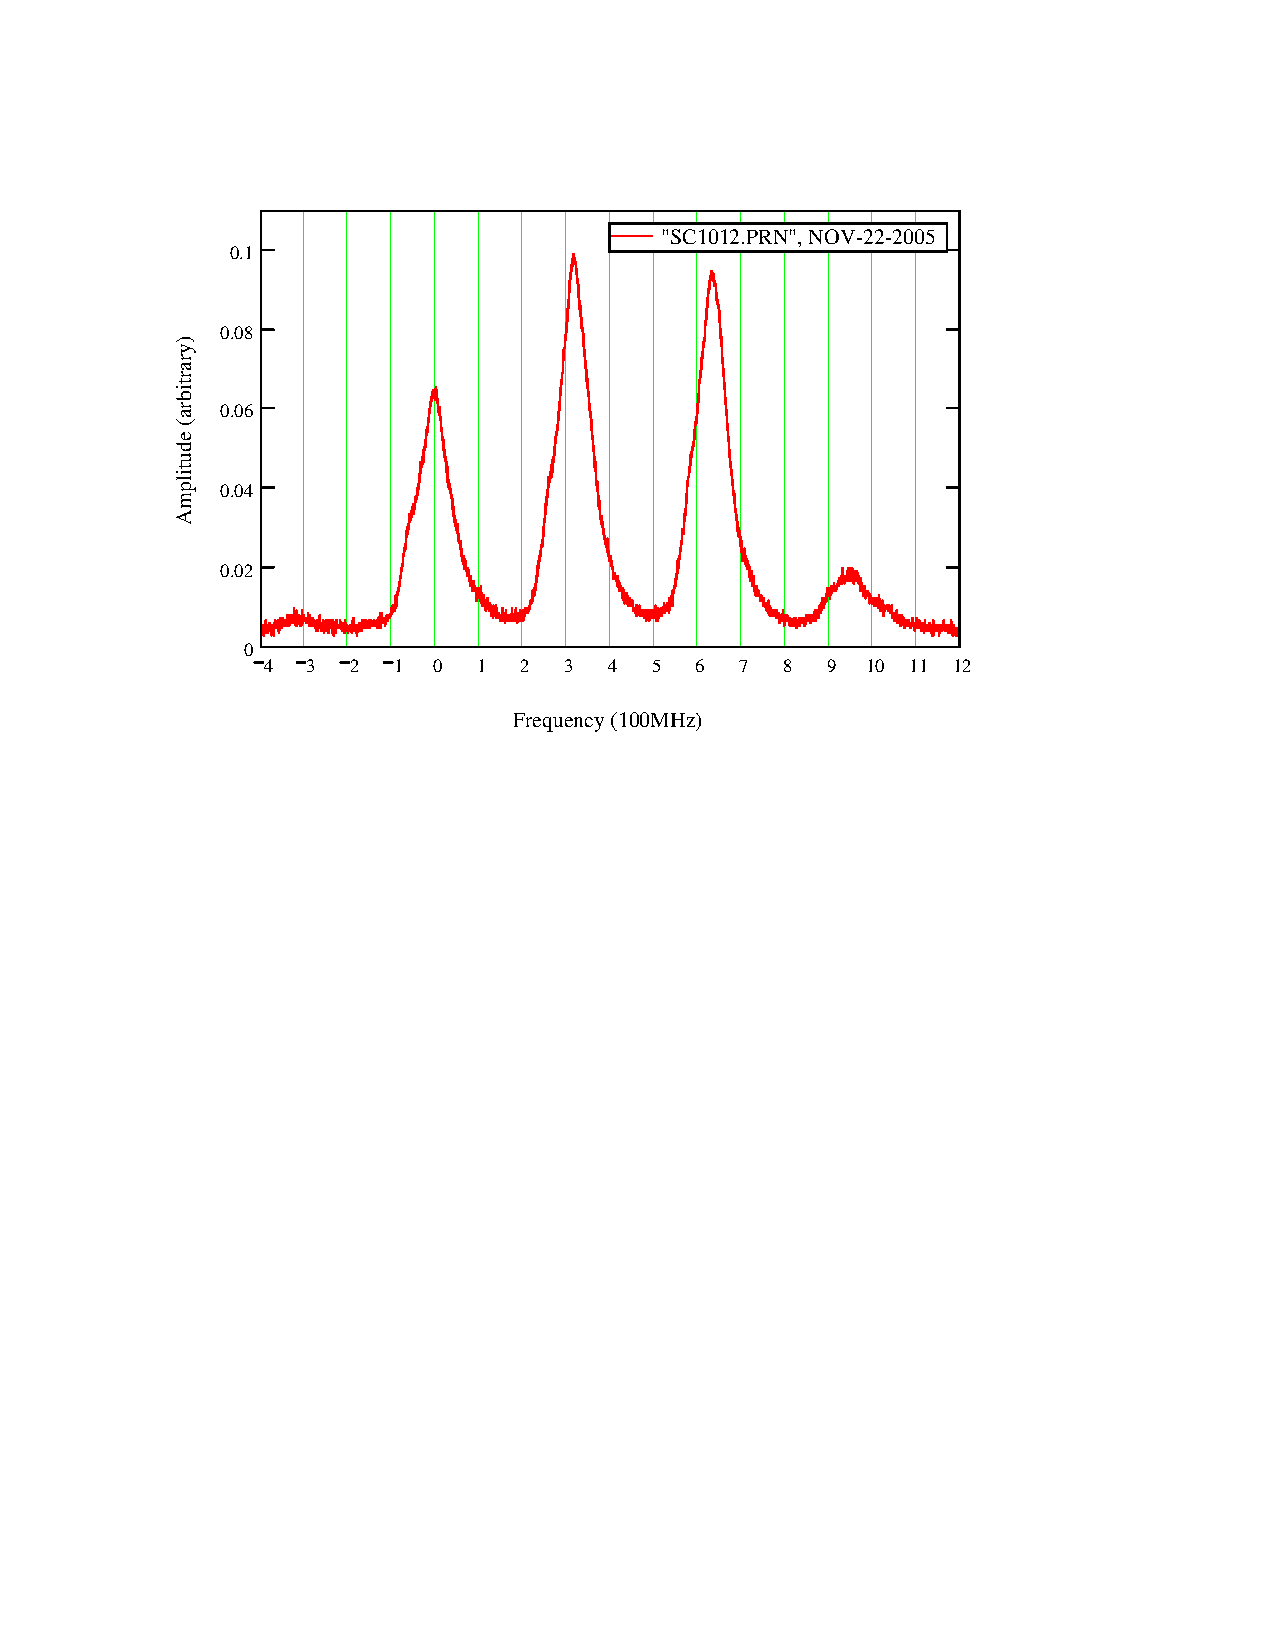
\includegraphics[bb=15 440 489 752]
{confocal_zoom/confocal_zoom.pdf}
}
\caption[Green HeNe transmission through a scanned confocal etalon (zoom)]{Green HeNe transmission through a scanned confocal etalon (zoom). The green HeNe mode spacing is 326 MHz and the etalon mode width is 100 MHz.}
\label{confocal_zoom}
\end{figure}
%----------------------------------------------------------------------------

%----------------------------------------------------------------------------
Optimal alignment for laser beam analysis is achieved when the half axial modes of confocal cavities can be identified and the full FSR of 16 GHz is apparent \cite{Siegman:1986a}. See Figure \ref{confocal_all} for a scope trace resulting from such an alignment. The maxima alternate in height with the tall peaks corresponding to the axial modes of the cavity and the short peaks the displaced odd transverse modes (the so called ``half axial'' modes). Within each maxima an inner structure is seen. Figure \ref{confocal_zoom} is a zoom into one of the axial peaks in the trace.

%----------------------------------------------------------------------------
%----------------------------------------------------------------------------
%bb defines the bounding box for the pdf
%viewport defines the area of the pdf used
%in sidewaysfigure the last entry in bb moves the caption toward/away the pic
%in sidewaysfigure the second entry in bb moves the pic toward/away the caption
%----------------------------------------------------------------------------
\begin{figure}
\scalebox{0.8}[0.8]{
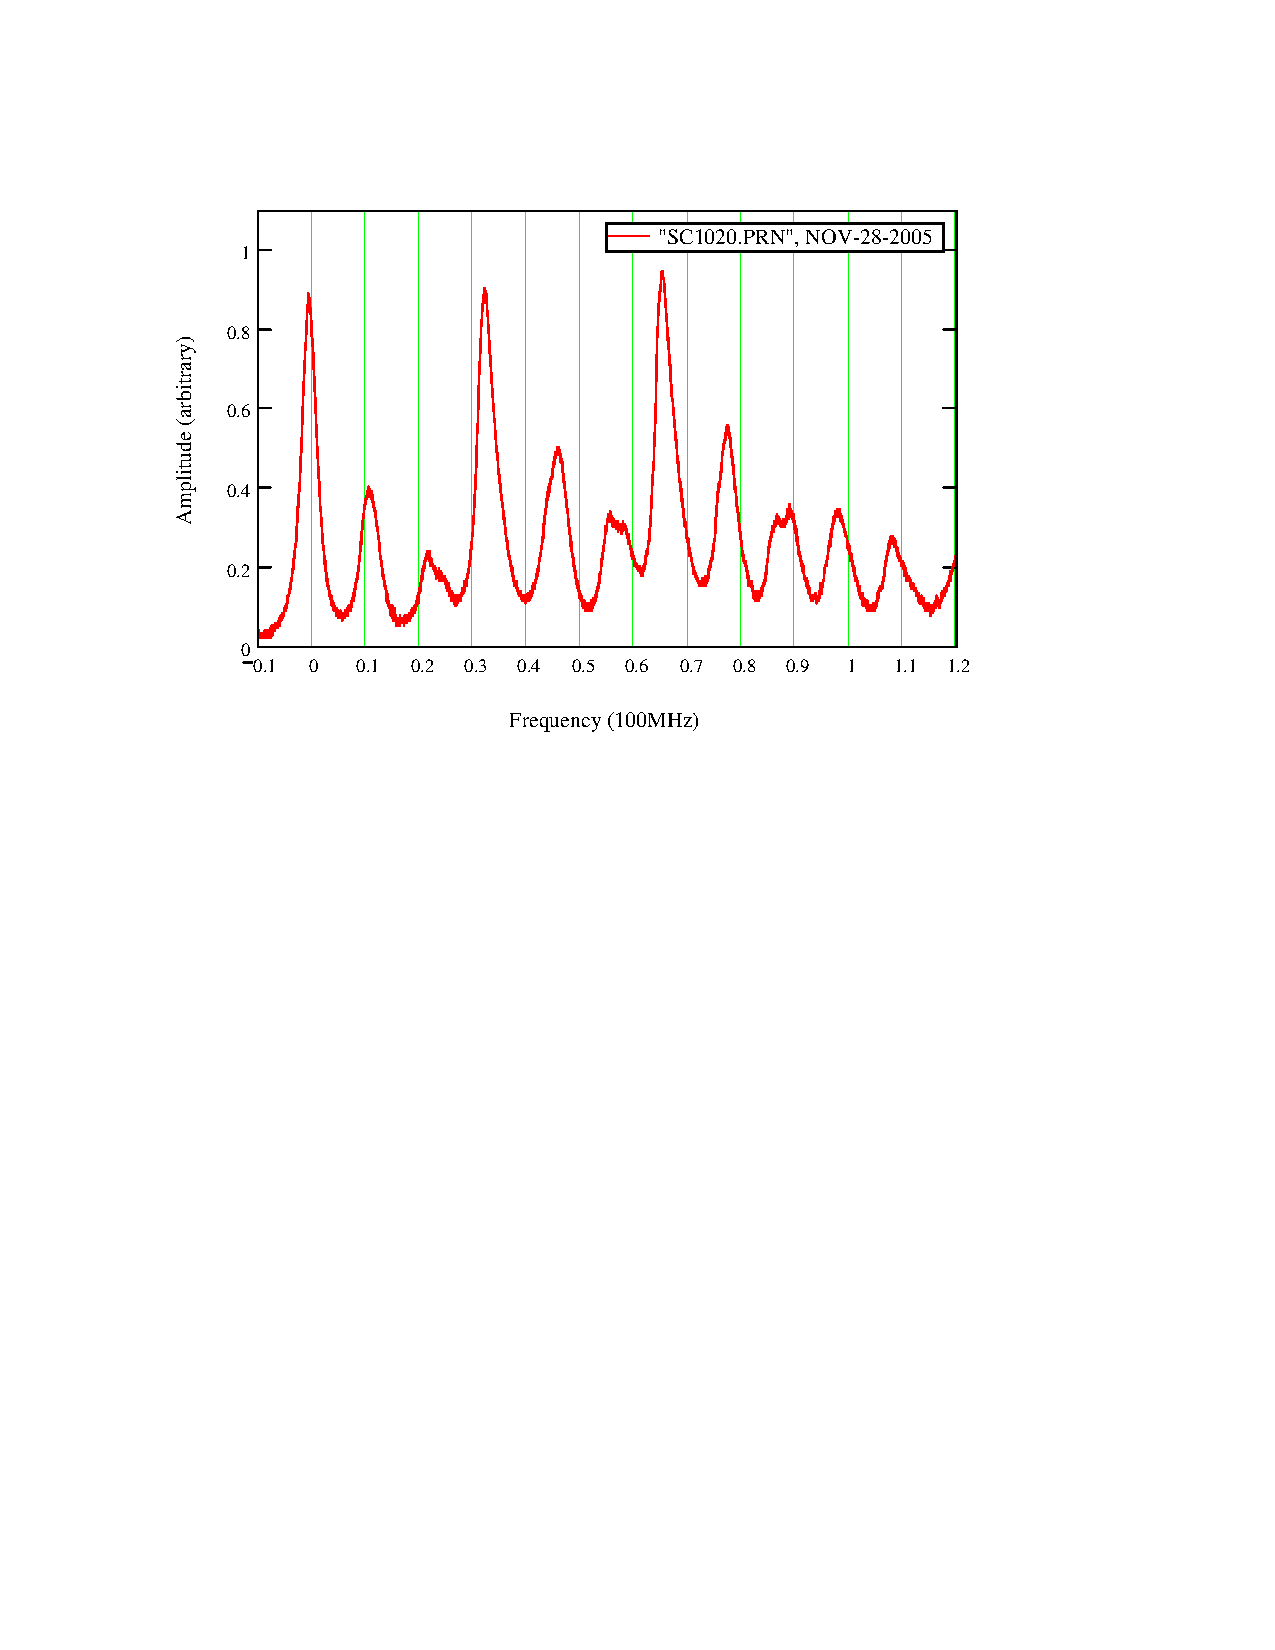
\includegraphics[bb=15 440 489 752]
{near_confocal/near_confocal.pdf}
}
\caption[Green HeNe transmission through a scaned near confocal etalon]{Green HeNe transmission through a scaned near confocal etalon}
\label{near_confocal}
\end{figure}
%----------------------------------------------------------------------------

%----------------------------------------------------------------------------
Figure \ref{near_confocal} show the output of the etalon when run in a ``near--confocal'' geometry. The etalon modes become non--degenerate and can be selected by adjusting the DC voltage to the piezo. When run in this mode with the TEM00 selected, the output of the etalon is not visible (even when focused) in room light.
%----------------------------------------------------------------------------
%----------------------------------------------------------------------------
